
\chapter{再随机化与回归调整}
 \label{chapter:rerandomization-regression}


第\ref{chapter::stratification-poststratification}章中提到的分层与后分层方法是针对随机实验设计与分析中离散协变量的处理手段。那么，面对多维且可能为连续的协变量时该如何处理呢？我们可以将连续协变量离散化，但这种方法在需要处理大量协变量时不甚理想。再随机化与回归调整正是针对一般协变量的处理手段，这也是本章要讨论的内容。 


下表总结了第\ref{chapter::stratification-poststratification}章与第\ref{chapter:rerandomization-regression}章所涉及的主题：


\begin{center}
\begin{tabular}{c|c|c}
\hline 
 & 实验设计 & 统计分析 \\ 
 \hline 
 离散协变量 & 分层法 & 后分层法 \\
 \hline 
 一般协变量 & 再随机化 & 回归调整 \\
 \hline 
 \end{tabular}
\end{center}





\section{再随机化}

\subsection{实验设计}
我们仍考虑一个包含 $n$ 个实验单元的有限总体，其中 $n_1$ 个单元接受处理，$n_0$ 个单元作为对照。设 $\bm{Z} = (Z_1,\ldots, Z_n)$ 为各实验单元的处理分配向量。每个单元 $i$ 都有一个协变量 $X_i \in \mathbb{R}^K$，其分量既可以是连续的也可以是二值的。我们将这些协变量整合为 $n\times K$ 的矩阵 $\bm{X} = (X_1 , \ldots, X_n )  \tran$，并将其均值中心化至零，即 $\bar{X}  = n^{-1} \sumn X_i = 0$ 以便简化后续推导。 

完全随机实验在平均意义上平衡处理组与对照组的协变量。例如，协变量均值差
$$
\hat{\tau}_X  = n_1^{-1} \sumn Z_i X_i - n_0^{-1} \sumn (1-Z_i) X_i
$$
在完全随机实验下的期望为零，但某次实际分配仍可能产生不理想的协变量平衡，即$\hat{\tau}_X  $的实现值往往不为零。利用习题\ref{hw::vector-neyman1923}中\citet{Neyman:1923}结论的向量形式，可得
$$
\cov(\hat{\tau}_X  ) 
= \frac{1}{n_1}  S_X^2  + \frac{1}{n_0}  S_X^2   
=  \frac{n}{n_1 n_0} S_X^2   ,
$$
其中$ S_X^2   = (n-1)^{-1} \sumn  X_i X_i\tran $是协变量的有限总体协方差矩阵。下面的马氏距离衡量两组差异：
\begin{equation}
\label{eq::m-distance-def}
M = \hat{\tau}_X \tran \cov(\hat{\tau}_X  )^{-1} \hat{\tau}_X  = \hat{\tau}_X \tran  \left(  \frac{n}{n_1 n_0} S_X^2   \right)^{-1} \hat{\tau}_X  . 
\end{equation}
严格地说，\eqref{eq::m-distance-def}中的$M$只有在$S_X^2 $可逆时才有意义，也就是协变量矩阵$\bm{X}$的列线性无关。若某列可由其他列线性表示，它就是冗余的，应在实验前删除。$M$的一个优点是对$X$的非退化线性变换不变。下面的引理\ref{lemma::invariance-mdistance}概括这一性质，证明留作习题\ref{para::invariance-M}。 

\begin{lemma}\label{lemma::invariance-mdistance}
若对所有单位$i=1,\ldots, n$，将$X_i$变换为$b_0  + BX_i$，其中$b_0  \in \mathbb{R}^K$且$B \in \mathbb{R}^{K\times K}$可逆，则\eqref{eq::m-distance-def}中的$M$保持不变。 
\end{lemma}




有限总体下的中心极限定理 \citep{li2017general} 表明：当实验样本量 $n$ 较大时，在完全随机化设计下，马氏距离 $M $ 近似服从 $ \chi^2_K$ 分布。这表明在完全随机化设计下 $M$ 的观测值通常较大，其渐进期望值为 $K$、方差为 $2K$。再随机化正是通过剔除那些 $M$ 值过大的处理方案来改善协变量平衡性。下面给出基于马氏距离的再随机化方法（简称 ReM）的正式定义，该方法由 \citet{cox:1982} 提出，后经 \citet{morgan2012rerandomization} 进一步研究完善。 


\begin{definition}
[ReM]
从完全随机实验中抽取$\bm{Z}$，并且仅当
$$
M \leq a,
$$
时接受该分配，其中$a > 0$是预先指定的常数。 
\end{definition}



选择$a$与选择分层随机实验的层数类似，在实践中并不容易。一个极端是$a = \infty$，这就是完全随机实验；另一个极端是$a=0$，此时可行分配很少，实验几乎失去随机性，基于随机化的推断也失去用途。折中的办法是选择较小但不极小的$a$，例如$a=0.001$，或$\chi^2_K$分布的某个分位数。 


 

ReM 具有诸多优良特性：如上所述，它对协变量的线性变换具有不变性；此外它还具有良好的几何性质与简洁的数学结构。本章后续将主要围绕 ReM 展开讨论。  


\subsection{统计推断}

再随机化后的数据应如何分析，是一个重要问题。\citet{bruhn2009pursuit}和\citet{morgan2012rerandomization}指出，只要在$M\leq a$的约束下模拟$\bm{Z}$，就始终可以使用 FRT；在尖锐零假设下，所得$p$值始终具有有限样本精确性，见习题\ref{hw::FRT-under-REM}。 


然而，若不对零假设做任何额外假设而直接推导再随机化的有限样本性质，则是极具挑战性的课题。\citet{li2018asymptotic} 在设定了若干正则条件后，导出了处理效应差 $\hat{\tau}$ 在再随机化下的渐进分布形式。



\begin{condition}\label{condition::regularity-cre-rem}
当总体样本量 $n\rightarrow \infty$ 时，必须满足以下条件：
\begin{enumerate}
\item 
处理组与对照组的样本比例 $n_1/n$ 与 $n_0/n$ 均收敛至一个大于零的有限值；
\item 
实验单元潜在结果 $\{  X_i, Y_i(1), Y_i(0), \tau_i \}$ 的有限总体协方差存在有限极限；
\item
$\max_{1\leq i \leq n}  \{   Y_i(1) - \bar{Y}(1) \} ^2/n \rightarrow 0 $， $\max_{1\leq i \leq n}  \{   Y_i(0) - \bar{Y}(0) \}^2/n \rightarrow 0 $，且 $\max_{1\leq i \leq n}   X_i \tran X_i/n \rightarrow 0 $。
\end{enumerate}
\end{condition} 


下面是再随机化的主要定理，需要先引入记号。令
$$
L_{K,a} \sim D_1\mid \bm{D}\tran \bm{D} \leq a
$$
其中$\bm{D} = (D_1,\ldots, D_K)$服从$K$维标准正态分布；令$ \varepsilon$服从一元标准正态分布，并令$L_{K,a}  \ind \varepsilon .$。


\begin{theorem}\label{thm::remasymptotics}
在满足$M\leq a$的再随机化设计及条件\ref{condition::regularity-cre-rem}下，有\footnote{记号“$A \asim B$”表示$A$与$B$具有相同的渐近分布。}
$$
\hat{\tau} - \tau \asim \sqrt{ \var(\hat \tau) }  \left\{   \sqrt{R^2} L_{K,a}  + \sqrt{1-R^2} \varepsilon \right\},
$$
其中
$$
\var( \hat{\tau} ) = \frac{S^2(1)}{n_1} + \frac{S^2(0)}{n_0} - \frac{S^2(\tau)}{n}
$$
是第\ref{chapter::neyman-cr}章证明的\citet{Neyman:1923}方差公式，
$$
R^2 = \textup{corr}^2(\hat{\tau}, \hat{\tau}_X   )
$$
是在完全随机实验下$\hat{\tau}$与$\hat{\tau}_X $之间的多重相关系数平方（定义见第\ref{sec::measure-pearson-r2}节）。
\end{theorem}


虽然\citet{li2018asymptotic}的证明涉及较多技术细节，定理\ref{thm::remasymptotics}中的渐近分布却有清楚的几何解释，见图\ref{fig::geometry-rem}：$\hat\tau$可分解为$\hat\tau_X$的线性组合与正交于$\hat\tau_X$的分量。几何上，$\cos^2 \theta = R^2$，其中$\theta$是$\hat\tau$与$\hat\tau_X$的夹角。再随机化影响第一个分量，而不改变第二个分量。截断正态分布$L_{K,a}$正是对第一个分量施加再随机化约束的结果。  


\begin{figure}
\centering
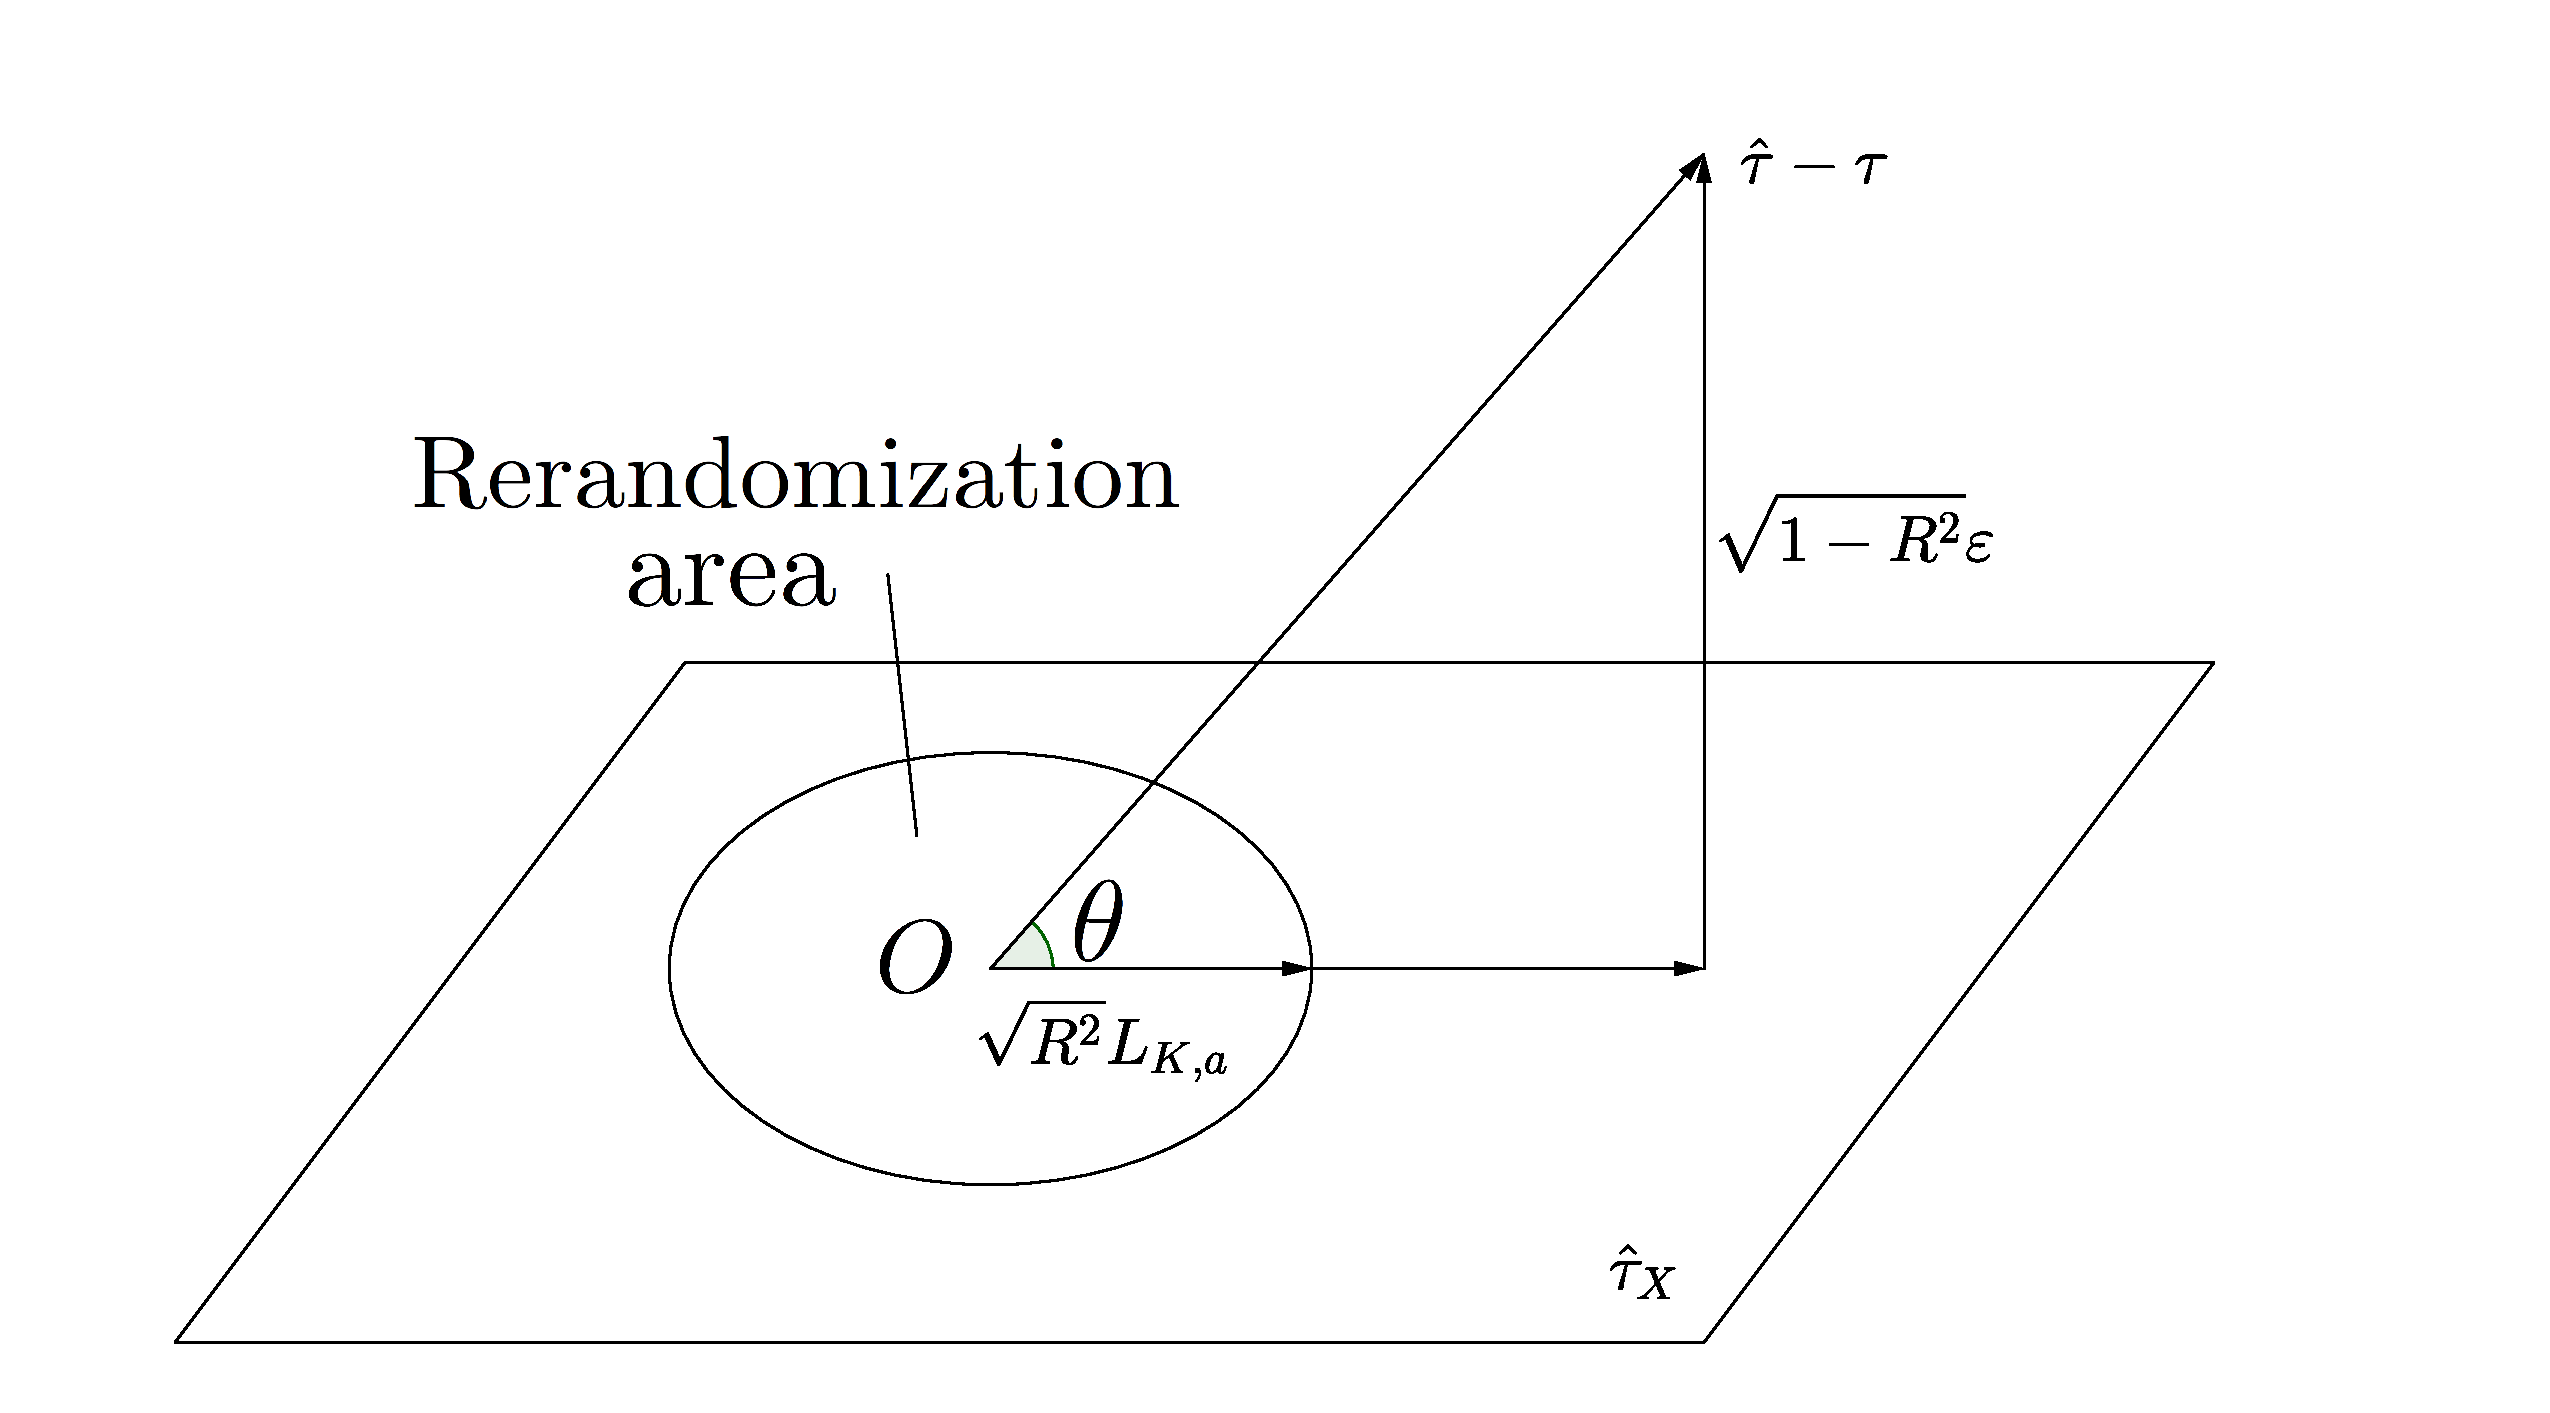
\includegraphics[width = 0.9\textwidth]{figures/rem_geometry.pdf}
\caption{再随机化下$\hat\tau$渐近分布的几何解释}\label{fig::geometry-rem}
\end{figure}


当阈值 $a  = \infty$ 时，该渐进分布退化为完全随机化下的分布形式：
$$
\hat{\tau} - \tau \asim \sqrt{ \var(\hat \tau) } \varepsilon .
$$
当阈值 $a$ 极接近于零时，分布形式变为：
$$
\hat{\tau} - \tau \asim \sqrt{ \var(\hat \tau) (1-R^2)} \varepsilon ;
$$
严格证明见 \citet{wang2022rerandomization}。由此可知，在 $a$ 值较小的情况下，再随机化的效率提升效果直接取决于 $R^2$ 的大小。该系数还具有以下等价表达形式。 
\begin{proposition}
\label{prop::rsquared-forms}
在完全随机实验下，
$$
R^2 = \textup{corr}^2(\hat{\tau}, \hat{\tau}_X   )
= \frac{  n_1^{-1}  S^2(1\mid X) + n_0^{-1} S^2(0\mid X) - n^{-1} S^2(\tau \mid X) }
{ n_1^{-1}  S^2( 1 ) + n_0^{-1} S^2( 0 ) - n^{-1} S^2( \tau  )},
$$
其中$\{S^2( 1 ) , S^2( 0 ), S^2( \tau  )\}$是$\{ Y_i(1), Y_i(0), \tau_i \}_{i=1}^n$的有限总体方差，$\{S^2( 1 \mid x ) , S^2( 0 \mid x ), S^2( \tau  \mid x )\}$是它们分别在线性空间$(1, X_i)$上投影后的有限总体方差；线性投影的定义见第\ref{sec::sampleOLS}节。 
%\footnote{For example, the linear projection of $Y_i(1)$ on $(1,X_i)$ is $\alpha_1 + \beta_1 X_i$ where 
%$$
%(\alpha_1, \beta_1) = \arg \min_{a,b} \sumn \{  Y_i(1) - a - b\tran X_i\}^2.
%$$
%}
在个体因果效应恒定、即$\tau_i = \tau$的假设下，$R^2 $简化为$S^2(0\mid X) / S^2( 0 ) $，也就是$Y_i(0)$与$X_i$的有限总体多重相关系数平方。
\end{proposition}

命题\ref{prop::rsquared-forms}的证明留作习题\ref{para::r2-cre}。 

当$ 0 < a <\infty$时，$\hat{\tau}$的渐近分布更复杂，却更集中在$\tau$附近，所以再随机化下的均值差$\hat{\tau}$比完全随机实验下更精确。 


若忽略再随机化设计，仍根据\cite{Neyman:1923}的方差公式和正态近似构造置信区间，即使个体因果效应恒定，区间也会过度保守，对$\tau$产生过高覆盖率。\citet{li2018asymptotic}提出根据定理\ref{thm::remasymptotics}构造置信区间。这里略去细节，第\ref{sec::unification-rem-regadj}节再回到推断问题。 
 



\section{回归调整}

当处理组与对照组样本量相等时，再随机化下的估计量偏差较小且渐进无偏；然而当两组样本量不等时，再随机化可能引入一定偏差。该点亦可从几何角度加以解释：在两组样本量不等时，正交分量的权重改变可能导致估计量方向调整幅度变大，从而引入更多偏差。 

\subsection{再随机化与后分层法的关联}\label{sec::covariate-adjusted-frt-intro}


协变量$\bm{X}$均为固定值；在$\HF$下，观测结果也全部固定。因此，可以模拟任意检验统计量$T = T(\bm{Z}, \bm{Y}, \bm{X})$的分布，并计算$p$值。有额外协变量时，FRT 的基本思想仍然不变。  


构造统计量有两种一般策略，此前习题\ref{hw::frt-covariates}已提示这两种思路。下面采用\citet{zhao2020caFRT}的术语作概括。 


\begin{definition}
[协变量调整 FRT 的伪结果策略]
\label{def::pseudo-y-frt}
可以根据统计模型拟合后的残差构造统计量。将$Y_i$对$X_i$作回归，得到残差$\hat \varepsilon_i$，然后将$\hat \varepsilon_i$视为伪结果来构造检验统计量。
\end{definition}



\begin{definition}
[协变量调整 FRT 的模型输出策略]
\label{def::model-out-frt}
可以将回归系数作为统计量。将$Y_i$对$(Z_i, X_i)$作回归，以$Z_i$的系数作为检验统计量。
\end{definition}

 

在定义\ref{def::pseudo-y-frt}的伪结果策略中，将$Y_i$对$X_i$作回归时不应加入处理$Z_i$，以保证原结果满足$\HF$时，伪结果也满足$\HF$。定义\ref{def::model-out-frt}的模型输出策略则在$Y_i$对$(Z_i, X_i)$的回归中加入处理$Z_i$，因为要用$Z_i$的系数衡量偏离$\HF$的程度。计算上，第一种策略只需回归一次，第二种策略则需反复回归。 

这里的“回归”泛指线性回归、逻辑回归，甚至机器学习算法。在$\HF$下，这两类策略产生的任意统计量都给出有限样本精确的 FRT，但在备择假设下表现可能不同。本节余下部分回顾若干基于 OLS 的统计量。 



\subsection{协方差分析及其推广}\label{sec::ancova}

现在转向直接估计平均因果效应$\tau$，并调整观测协变量。 

历史上，\citet{fisher1925statistical}提出用协方差分析（ANCOVA）提高估计效率。它至今仍是许多领域的标准方法：将$Y_i$对$(1, Z_i, X_i)$作 OLS 回归，取$Z_i$的系数估计$\tau$。将 Fisher 的 ANCOVA 估计量记为$\hat{\tau}_\textsc{F}$。 


曾任伯克利统计系教授的 David A. Freedman 在\citet{Neyman:1923}的潜在结果框架下重新分析了 Fisher 的 ANCOVA。\citet{freedman2008regression_a, freedman2008regression_b}发现以下负面结果：
\begin{enumerate}
[(1)]
\item
$\hat{\tau}_\textsc{F}$有偏，而简单均值差$\hat{\tau}$无偏。
\item 
当$n_1\neq n_0$时，$\hat{\tau}_\textsc{F}$的渐近方差甚至可能大于$\hat{\tau}$的渐近方差。
\item 
在完全随机实验下，OLS 给出的标准误不是$\hat{\tau}_\textsc{F}$真实标准误的一致估计。   
\end{enumerate}


曾在伯克利攻读博士的 Winston Lin 在论文中回应了 Freedman 的批评。\citet{lin2013}得到了以下正面结论：
\begin{enumerate}
[(1)]
\item
大样本下，$\hat{\tau}_\textsc{F}$的偏差较小，并随着样本量趋于无穷而趋于零。
\item
将$Y_i$对$(1, Z_i, X_i, Z_i\times X_i)$作 OLS 回归，以$Z_i$的系数作为估计量，可以同时改进$\hat{\tau}$与$\hat{\tau}_\textsc{F}$的渐近效率。用$\hat{\tau}_\textsc{L}$表示\citet{lin2013}的估计量。此外，EHW 标准误是在完全随机实验下$\hat{\tau}_\textsc{L}$真实标准误的保守估计。 
\item
将$Y_i$对$(1, Z_i, X_i)$作 OLS 回归时，$\hat{\tau}_\textsc{F}$的 EHW 标准误\footnote{不含协变量时，HC2 修正得到的方差估计与\citet{Neyman:1923}的经典估计完全相同，见习题\ref{hw::neyman-ols-nox}。为统一处理，也可以对\citet{lin2013}的协变量调整估计量使用 HC2 修正。当协变量数相对样本量较小、且协变量无离群值时，EHW 标准误的不同变体表现相近；协变量较多或存在离群值时，变体可能优于原方法。此时\citet{lei2018regression}推荐 HC3 变体。}是在完全随机实验下$\hat{\tau}_\textsc{F}$真实标准误的保守估计。 
\end{enumerate}


\subsubsection{\citet{lin2013}结论的直观解释}


\citet{Neyman:1923}的结论表明，均值差估计量$\hat{\tau}$的方差依赖于潜在结果的方差。直观上，降低潜在结果的方差，就能降低估计量的方差。考虑一类线性调整估计量
\begin{eqnarray} 
\hat{\tau}(\beta_1, \beta_0) &=& n_1^{-1} \sumn Z_i(Y_i - \beta_1\tran X_i) - n_0^{-1} \sumn (1-Z_i) (Y_i - \beta_0\tran X_i)  \label{eq::linear-adj-1}\\
&=& \left\{  \hat{\bar{Y}}(1) - \beta_1\tran \hat{\bar{X} }(1) \right\}  -  \left\{   \hat{\bar{Y}}(0) - \beta_0\tran \hat{\bar{X} }(0) \right\},
\label{eq::linear-adj-2}
\end{eqnarray}
其中$\{ \hat{\bar{Y}}(1), \hat{\bar{Y}}(0) \}$为结果的样本均值，$\{ \hat{\bar{X} }(1), \hat{\bar{X} }(0)\}$为协变量的样本均值。估计量$\hat{\tau}(\beta_1, \beta_0)$通过对潜在结果残差化来降低$\hat\tau$的方差；取$\beta_1 = \beta_0 = 0$时，它退化为$\hat\tau$。由于$\bar{X}  = 0.$，对任意固定$\beta_1$和$\beta_0$，其期望都为$\tau$。我们希望选择$(\beta_1, \beta_0)$，使$\hat{\tau}(\beta_1, \beta_0)$的方差最小。这本质上是调整后潜在结果$\{ Y_i(1) - \beta_1\tran X_i  , Y_i(0) - \beta_0\tran  X_i \}_{i=1}^n $的均值差。应用\citet{Neyman:1923}的结论，方差为
$$
\var\{ \hat{\tau}(\beta_1, \beta_0) \} = \frac{ {S}^2(1; \beta_1) }{ n_1 } + \frac{ {S}^2(0; \beta_0) }{ n_0 }
- \frac{  S^2(\tau; \beta_1, \beta_0)  }{ n },
$$
其中$ {S}^2(z; \beta_z)$（$(z=1,0)$）与$S^2(\tau; \beta_1, \beta_0)$分别为调整后潜在结果及个体因果效应的有限总体方差；保守方差估计为
$$
\hat{V}( \beta_1, \beta_0 ) = \frac{ \hat{S}^2(1; \beta_1) }{ n_1 } + \frac{ \hat{S}^2(0; \beta_0) }{ n_0 },
$$
其中
\begin{eqnarray*}
\hat{S}^2(1; \beta_1) &=& (n_1-1)^{-1} \sumn Z_i  ( Y_i - \gamma_1 - \beta_1\tran  X_i )^2,\\ 
\hat{S}^2(0; \beta_0) &=& (n_0-1)^{-1} \sumn (1-Z_i)  ( Y_i - \gamma_0 - \beta_0\tran  X_i )^2
\end{eqnarray*}
是调整后潜在结果的样本方差，$\gamma_1$、$\gamma_0$分别是处理组中$Y_i - \beta_1\tran  X_i$与对照组中$Y_i   - \beta_0\tran  X_i $的样本均值。要使$\hat{V}( \beta_1, \beta_0 )$最小，需要求解两个 OLS 问题\footnote{也可最小化$\hat{\tau}(\beta_1, \beta_0) $的真实方差，详见习题\ref{hw::compare-true-variance}。}：
$$
\min_{\gamma_1 , \beta_1 }
\sumn Z_i  ( Y_i - \gamma_1 - \beta_1\tran  X_i )^2,\quad
\min_{\gamma_0 , \beta_0 }
\sumn (1-Z_i)  ( Y_i - \gamma_0 - \beta_0\tran  X_i  )^2.
$$
分别在处理组和对照组将$Y_i$对$X_i$作 OLS 回归，得到$( \hat{\gamma}_1, \hat{\beta}_1 )$和$( \hat{\gamma}_0, \hat{\beta}_0 )$。最终估计量为
\begin{eqnarray*}
 \hat{\tau}( \hat{\beta}_1, \hat{\beta}_0) &=& n_1^{-1} \sumn Z_i(Y_i - \hat{\beta}_1\tran  X_i) 
- n_0^{-1} \sumn (1-Z_i)  (Y_i - \hat{\beta}_0\tran  X_i) \\
&=&\left\{  \hat{\bar{Y}}(1) - \hat \beta_1\tran \hat{\bar{X} }(1) \right\}  
-  \left\{   \hat{\bar{Y}}(0) - \hat \beta_0\tran \hat{\bar{X} }(0) \right\} . 
\end{eqnarray*}
由 OLS 拟合的性质（见\eqref{eq::OLS-mean-data}），
$$
\hat{\bar{Y}}(1) =  \hat{\gamma}_1 + \hat{\beta}_1\tran  \hat{\bar{X} }(1),\quad
\hat{\bar{Y}}(0) =  \hat{\gamma}_0 + \hat{\beta}_0\tran  \hat{\bar{X} }(0).
$$
故可将估计量改写为
\begin{equation}
\label{eq::lin-intercepts}
 \hat{\tau}( \hat{\beta}_1, \hat{\beta}_0)  =  \hat{\gamma}_1 - \hat{\gamma}_0  
\end{equation}
\eqref{eq::lin-intercepts}中的等价形式表明，$ \hat{\tau}( \hat{\beta}_1, \hat{\beta}_0) $也可以通过下面的一次 OLS 回归得到。




\begin{proposition}\label{prop::lin-ols}
\eqref{eq::lin-intercepts}中的估计量$ \hat{\tau}( \hat{\beta}_1, \hat{\beta}_0) $，等于将$Y_i$对$(1, Z_i, X_i, Z_i\times X_i)$作 OLS 回归得到的$Z_i$系数，即此前介绍的\citet{lin2013}估计量$\hat{\tau}_\textsc{L}$。 
\end{proposition}

命题\ref{prop::lin-ols}是一个纯粹的线性代数事实，证明留作习题\ref{para::lin-ols-covadj}。 


根据以上讨论，$\hat{\tau}_\textsc{L}$的保守方差估计量为
\begin{eqnarray*}
\hat{V}(  \hat{\beta}_1, \hat{\beta}_0 ) 
%= \frac{ \hat{S}^2(1; \hat{\beta}_1) }{ n_1 } + \frac{ \hat{S}^2(0; \hat{\beta}_0) }{ n_0 }
&=& \frac{1}{n_1(n_1 - 1)} \sumn Z_i  ( Y_i - \hat{\gamma}_1 - \hat{\beta}_1\tran  X_i  ) ^2 \\
&& \qquad + \frac{1}{n_0(n_0 - 1)} \sumn (1-Z_i)  ( Y_i - \hat{\gamma}_0 - \hat{\beta}_0\tran  X_i )^2.
\end{eqnarray*}
\citet{lin2013}通过较复杂的推导进一步证明，命题\ref{prop::lin-ols}中 OLS 回归给出的 EHW 标准误，与由$\hat{V}(  \hat{\beta}_1, \hat{\beta}_0 ) $计算的标准误几乎相同，后者是在完全随机实验下$\hat{\tau}_\textsc{L}$真实标准误的保守估计。直观上，这是因为我们未假定线性模型设定正确，而 EHW 标准误对模型误设具有稳健性。 



上述讨论有一个微妙之处：方差公式$\var\{ \hat{\tau}(\beta_1, \beta_0) \} $适用于固定$(\beta_1, \beta_0)$，而估计量$ \hat{\tau}( \hat{\beta}_1, \hat{\beta}_0) $使用了两个估计系数$( \hat{\beta}_1, \hat{\beta}_0) $。估计系数的额外不确定性可能使最终估计量产生有限样本偏差。\citet{lin2013}证明，这一问题在渐近意义下消失，因为$ \hat{\tau}( \hat{\beta}_1, \hat{\beta}_0) $与$ \hat{\tau}( \tilde{\beta}_1, \tilde{\beta}_0) $表现相似，其中$\tilde{\beta}_1$、$\tilde{\beta}_0$分别是$\hat{\beta}_1$、$ \hat{\beta}_0$的极限。直观上，$ \hat{\tau}( \hat{\beta}_1, \hat{\beta}_0) $与$ \hat{\tau}( \tilde{\beta}_1, \tilde{\beta}_0) $之差依赖于
$$
(\hat{\beta}_z - \tilde{\beta}_z)\tran \hat{\bar{X} }(z) ,\quad (z=0,1) 
$$
它是两个小阶量的乘积。需要注意，渐近理论要求较大样本量，以及潜在结果和协变量满足一定正则条件。在有限样本中，$\hat{\beta}_1$和$\hat{\beta}_0$估计带来的额外不确定性甚至可能使回归调整有害。 




\subsubsection{通过预测潜在结果理解\citet{lin2013}的估计量}
\label{sec::understand-lin-predict}
 
\begin{table}
\centering
\caption{再随机化与协变量不平衡的调整}\label{tb::predict-po-ols}
\begin{tabular}{cccccc}
\hline 
$X$ & $Z$ & $Y(1)$ & $Y(0)$ &  $\hat{Y}(1)$ & $\hat{Y}(0)$ \\
\hline
$X_1 $ & 1 & $Y_1(1)$ & ? & $\hat{\mu}_1(X_1 )$ & $\hat{\mu}_0(X_1)$ \\
\vdots \\
$X_{n_1}$ & 1 & $Y_{n_1}(1)$ & ? & $\hat{\mu}_1(X_{n_1})$ & $\hat{\mu}_0(X_{n_1})$ \\
$X_{n_1 + 1}$ & 0 & ? & $Y_{n_1+1}(0)$ & $\hat{\mu}_1(X_{n_1+1})$ & $\hat{\mu}_0(X_{n_1+1})$ \\
\vdots \\
$X_{n}$ & 0 & ? & $Y_{n}(0)$ & $\hat{\mu}_1(X_{n})$ & $\hat{\mu}_0(X_{n})$ \\
\hline 
\end{tabular}
\end{table}


 
可以把\citet{lin2013}的估计量看作基于潜在结果对协变量 OLS 拟合的{\it 预测型估计量}。用处理组数据，建立由$X$预测$Y(1)$的模型：
\begin{eqnarray}
\label{eq::pred-y1-linear}
\hat{\mu}_1(X) = \hat{\gamma}_1 + \hat{\beta}_1\tran X.
\end{eqnarray}
类似地，用对照组数据，建立由$X$预测$Y(0)$的模型：
\begin{eqnarray}
\label{eq::pred-y0-linear}
\hat{\mu}_0(X)= \hat{\gamma}_0 + \hat{\beta}_0\tran X . 
\end{eqnarray}
表\ref{tb::predict-po-ols}说明潜在结果的预测。若只预测缺失的潜在结果，可得预测型估计量
\begin{eqnarray}\label{eq::predictive-estimator-generic}
\hat{\tau}_\text{pred} = n^{-1} \left\{   \sum_{Z_i=1}Y_i + \sum_{Z_i=0}\hat{\mu}_1(X_i) - \sum_{Z_i=1} \hat{\mu}_0(X_i) - \sum_{Z_i=0} Y_i     \right\} .
\end{eqnarray}
可验证，采用\eqref{eq::pred-y1-linear}与\eqref{eq::pred-y0-linear}时，这个预测型估计量等于\citet{lin2013}的估计量：
\begin{eqnarray}
\label{eq::predictiveestimator}
\hat{\tau}_\text{pred} = \hat{\tau}_\textsc{L}.
\end{eqnarray}
若预测所有潜在结果，包括已经观测到的结果，则得到{\it 投影型估计量}：
\begin{eqnarray}\label{eq::projective-estimator-generic}
\hat{\tau}_\text{proj} = n^{-1}  \sumn \{ \hat{\mu}_1(X_i) - \hat{\mu}_0(X_i)    \}.
\end{eqnarray}
可验证，采用\eqref{eq::pred-y1-linear}与\eqref{eq::pred-y0-linear}时，投影型估计量也等于\citet{lin2013}的估计量：
\begin{eqnarray}
\label{eq::projectiveestimator}
\hat{\tau}_\text{proj} = \hat{\tau}_\textsc{L}.
\end{eqnarray}
\eqref{eq::predictiveestimator}与\eqref{eq::projectiveestimator}的证明留作习题\ref{para::predictiveestimator}。 


“预测型”与“投影型”的术语来自抽样调查文献\citep{firth1998robust, ding2018causal}。在更一般的公式\eqref{eq::predictive-estimator-generic}和\eqref{eq::projective-estimator-generic}中，也可使用其他潜在结果预测器。为说明与\citet{lin2013}估计量的联系，这里采用线性预测。预测器$\hat{\mu}_1(X)$与$\hat{\mu}_0(X)$可以非常一般，包括更复杂的机器学习算法。但构造点估计只是分析完全随机实验的第一步，更重要的第二步是量化估计量的不确定性，这取决于潜在结果预测器的性质。不过，无需额外理论分析，总可将\eqref{eq::predictive-estimator-generic}和\eqref{eq::projective-estimator-generic}作为 FRT 的检验统计量。 
 
 
\subsubsection{通过调整协变量不平衡理解\citet{lin2013}的估计量}
\label{sec::lin=adjustingforimbalance}

线性调整估计量可等价地写成
\begin{eqnarray}\label{eq::linear-covariate-imbalance}
%\hat{\tau}(\gamma) = 
\hat{\tau}(\beta_1, \beta_0) = \hat{\tau} - \gamma\tran \hat{\tau}_X 
\end{eqnarray}
其中$\gamma =\frac{n_0}{n} \beta_1 + \frac{n_1}{n} \beta_0$，因而也可写为$\hat{\tau}(\gamma) = 
\hat{\tau}(\beta_1, \beta_0) .$。类似地，\citet{lin2013}的估计量有等价形式
\begin{eqnarray}\label{eq::lin-covariate-imbalance}
\hat{\tau}_\textsc{L} = \hat{\tau} - \hat \gamma\tran \hat{\tau}_X ,
\end{eqnarray}
其中$\hat \gamma =\frac{n_0}{n} \hat \beta_1 + \frac{n_1}{n} \hat  \beta_0$。\eqref{eq::linear-covariate-imbalance}与\eqref{eq::lin-covariate-imbalance}的证明留作习题\ref{para::reg-covariate-imbalance}。\eqref{eq::linear-covariate-imbalance}与\eqref{eq::lin-covariate-imbalance}正是“调整协变量不平衡”的数学表达：从原均值差中减去协变量均值差的某个线性组合。在完全随机实验下，$\hat{\tau} $与$\hat{\tau}_X $相关，因此适当选择$\gamma$作协变量调整，就可降低$\hat{\tau} $的方差。\eqref{eq::linear-covariate-imbalance}和\eqref{eq::lin-covariate-imbalance}还有一个有意思的性质：最终估计量只依赖$\gamma$或$\hat \gamma$，因此$\beta$系数的选择并不唯一。\citet{li2019rerandomization}指出了这一简单事实。所以，\citet{lin2013}的估计量只是最优估计量之一；但它容易通过标准 OLS 与 EHW 标准误实现，因此本书主要介绍它。 



\subsection{关于回归调整的补充说明}


\subsubsection{再随机化与回归调整的对偶性}\citet{li2018asymptotic}指出，再随机化与\citet{lin2013}的回归调整分别在实验设计阶段和分析阶段使用协变量，二者具有对偶关系。具体而言，$a$较小时，再随机化下$\hat{\tau}$的渐近分布与完全随机实验下$\hat{\tau}_\textsc{L}$的渐近分布几乎相同。因此，再随机化在设计阶段使用协变量，\citet{lin2013}的回归调整在分析阶段使用协变量；当$a$较小时，二者几乎取得相同的渐近效率增益。 


 \subsubsection{回归调整与后分层的等价性}若离散协变量$C_i$有$K$个类别，可构造$K-1$个中心化的虚拟变量
$$
X_i = ( I(C_i=1) - \pi_{[1]}, \ldots,   I(C_i=K-1) - \pi_{[K-1]})
$$
其中$\pi_{[k]}$为满足$C_i = k$的单位比例。此时\citet{lin2013}的回归调整等价于后分层，见下面的命题。 

\begin{proposition}
\label{prop::lin=ps-discrete}
基于$X_i$的$\hat{\tau}_\textsc{L}$与基于$C_i$的后分层估计量$\hat{\tau}_\textsc{PS}$在数值上完全相同（见第\ref{sec::poststra-cre}节）。 
\end{proposition}


命题\ref{prop::lin=ps-discrete}的证明留作习题\ref{para::lin=ps-discrete}。 


\subsubsection{作为协变量调整$\hat \tau(\beta_1, \beta_0)$特例的双重差分}\label{sec::difference-in-difference-CRE}
许多研究中的重要协变量$X$是处理前的滞后结果。例如，教育研究中，结果$Y$是后测成绩，协变量$X$是前测成绩；职业培训研究中，结果$Y$是培训后的对数工资，协变量$X$是培训前的对数工资。以滞后结果$X$为协变量，一种常用方法是{\it 增益分数}或{\it 双重差分}估计量，即在\eqref{eq::linear-adj-1}和\eqref{eq::linear-adj-2}中固定$\beta_1 = \beta_0=1$：
\begin{eqnarray*}
\hat{\tau}(1,1) &=& n_1^{-1} \sumn Z_i(Y_i -   X_i) - n_0^{-1} \sumn (1-Z_i) (Y_i -   X_i) \\
&=& \left\{   \hat{\bar{Y}}(1) - \hat{\bar{Y}}(0) \right\} -  \left\{   \hat{\bar{X} }(1) - \hat{\bar{X} }(0) \right\} .
\end{eqnarray*}
$\hat{\tau}(1,1) $的第一种形式说明了{\it 增益分数}这一名称，因为它本质上是增益分数$g_i = Y_i - X_i$的均值差。$\hat{\tau}(1,1) $的第二种形式说明了{\it 双重差分}这一名称，因为它是两个均值差之差。它不同于\citet{lin2013}的估计量：它事先固定$\beta_1 = \beta_0=1$，而\citet{lin2013}的估计量需要估计两个$\beta$。$\hat{\tau}(1,1) $是无偏的，其保守方差估计量为
\begin{eqnarray*}
\hat{V}( 1,1 ) 
&=& \frac{1}{n_1(n_1 - 1)} \sumn Z_i  \{ g_i - \hat{\bar{g}}(1)   \}^2 \\
& & \qquad + \frac{1}{n_0(n_0 - 1)} \sumn (1-Z_i)  \{ g_i - \hat{\bar{g}}(0)   \}^2,
\end{eqnarray*}
其中$\hat{\bar{g}}(1)$和$ \hat{\bar{g}}(0)$分别为处理组与对照组的增益分数$g_i = Y_i - X_i$的样本均值。若滞后结果能很好地预测结果，增益分数$g_i = Y_i - X_i$的方差往往远小于结果本身的方差；此时$\hat{\tau}(1,1) $能显著降低简单结果均值差的方差。详见习题\ref{hw::did-CRE}。 


理论上，在大样本中，\citet{lin2013}的估计量始终比$\hat{\tau}(1,1)$更有效率。但\citet{lin2013}的估计量有有限样本偏差，而$\hat{\tau}(1,1)$始终无偏。   





\subsection{推广到分层随机实验}\label{sec::covariate-SRE}


实验可能按离散变量$C$分层，同时观测到额外协变量$X$。若每层都足够大，可在层内计算\citet{lin2013}的估计量$\hat{\tau}_{\textsc{L},[k]}$，再合成为
$$
\hat{\tau}_{\textsc{L},\textsc{S}} = \sum_{k=1}^K \pi_{[k]} \hat{\tau}_{\textsc{L},[k]} . 
$$
保守方差估计量为
$$
\hat{V}_{\textsc{L},\textsc{S}} =  \sum_{k=1}^K \pi_{[k]}^2 \hat{V}_{\textsc{ehw},[k]},
$$
其中$\hat{V}_{\textsc{ehw},[k]}$是在第$k.$层内，将结果对截距、处理指标、协变量及处理与协变量交互项作 OLS 回归得到的 EHW 方差估计。协变量必须按各层自己的均值进行中心化。
 

\section{统一、组合与比较}
\label{sec::unification-rem-regadj}


\citet{li2019rerandomization}统一了相关文献，证明再随机化可以与回归调整结合：在设计阶段进行再随机化后，分析阶段可使用\citet{lin2013}的估计量及 EHW 标准误。这种结合既改善设计阶段的协变量平衡，也提高分析阶段的估计效率。 




表\ref{tb::rerandomization-regression}概括了从\citet{Neyman:1923}到\citet{li2019rerandomization}的研究。箭头 1 表示完全随机实验中协变量调整的效率增益：渐近地，$\hat\tau_\textsc{L}$的方差小于$\hat\tau$。箭头 2 表示再随机化的效率增益：渐近地，$\hat{\tau}$在再随机化下的分位区间窄于完全随机实验。箭头 3 和 4 表示将再随机化与回归调整相结合的收益。



\begin{table}
\centering
\caption{随机实验的设计与统计分析}\label{tb::design-analysis-2x2}
\label{tb::rerandomization-regression}
\begin{tabular}{c|cccc}
\hline 
  & & & 统计分析 & \\
  \hline 
  & CRE & $\hat\tau$ \citep{Neyman:1923} &  $\stackrel{1}{\longrightarrow}$  &  $\hat\tau_\textsc{L}$ \citep{lin2013} \\
  实验设计&  &  $2\Big\downarrow$ && $  \Big\downarrow 4$ \\
  & 再随机化 & $\hat\tau$  \citep{li2018asymptotic} &  $\stackrel{3}{\longrightarrow}$  &$\hat\tau_\textsc{L}$ \citep{li2019rerandomization}  \\
  \hline 
\end{tabular}
\end{table}



 

\section{模拟}
\label{sec::rem-reg-simulation}

\citet{angrist2009incentives}在加拿大某大学开展实验，评价提高一年级学生学业表现的不同策略。这里使用原数据的一个子集，比较对照组与同时获得学业支持服务及良好成绩经济奖励的处理组。结果是第一学年末的 GPA。缺失结果以观测均值填补，这种做法有一定任意性（见习题\ref{hw::missing-y-experiments}）。两个协变量为性别和基线 GPA。

\begin{lstlisting}
angrist   = read.dta("star.dta")
angrist2  = subset(angrist, control == 1||sfsp == 1)
## imputing missing outcomes
y = angrist2$GPA_year1
meany    = mean(y, na.rm = TRUE)
y = ifelse(is.na(y), meany, y)
z = angrist2$sfsp 
x = angrist2[, c("female", "gpa0")]
\end{lstlisting}


以下代码演示了两种估计量的统计性质： 
\begin{lstlisting}
> ## unadjusted estimator
> fit_unadj = lm(y ~ z)
> ace_unadj = coef(fit_unadj)[2]
> se_unadj  = sqrt(hccm(fit_unadj, type = "hc2")[2, 2])
> 
> ## regression adjustment
> x         = scale(x)
> fit_adj   = lm(y ~ z*x)
> ace_adj   = coef(fit_adj)[2]
> se_adj    = sqrt(hccm(fit_adj, type = "hc2")[2, 2])
> 
> res = c(ace_unadj, ace_adj, se_unadj, se_adj)
> dim(res) = c(2, 2)
> t.stat   = res[, 1]/res[, 2]
> p.value  = 2*pnorm(abs(t.stat), lower.tail = FALSE) 
> res      = cbind(res, t.stat, p.value)
> rownames(res) = c("Neyman", "Lin")
> colnames(res) = c("estimate", "s.e.", "t-stat", "p-value")
> round(res, 3)
       estimate  s.e. t-stat p-value
Neyman    0.054 0.076  0.719   0.472
Lin       0.075 0.072  1.036   0.300
\end{lstlisting}
尽管回归调整估计量的标准误小于原始估计量，二者在统计显著性层面并无显著差别。 



还利用此数据集模拟比较表\ref{tb::design-analysis-2x2}中的四种设计与分析策略。分别在处理组和对照组，用结果对协变量拟合二次函数，填补所有缺失潜在结果。为展示再随机化和回归调整的改进，还分别将误差项乘以$0.1$和$0.25$，提高信噪比。利用填补后的科学表，生成 2000 次处理分配，得到观测数据并计算估计量。模拟中的“真实”结果模型非线性，但仍采用线性调整估计，以评价线性模型误设时估计量的性质。 


图\ref{fg::rerandomizationandancova}给出了四种组合的估计值减去真实$\tau$后的小提琴图。\footnote{小提琴图类似箱线图，但两侧各增加一幅旋转后的核密度图。}正如理论预测，所有估计量都近似无偏，再随机化和回归调整均提高效率，而且噪声越小，效果越明显。 

\begin{figure}
\centering
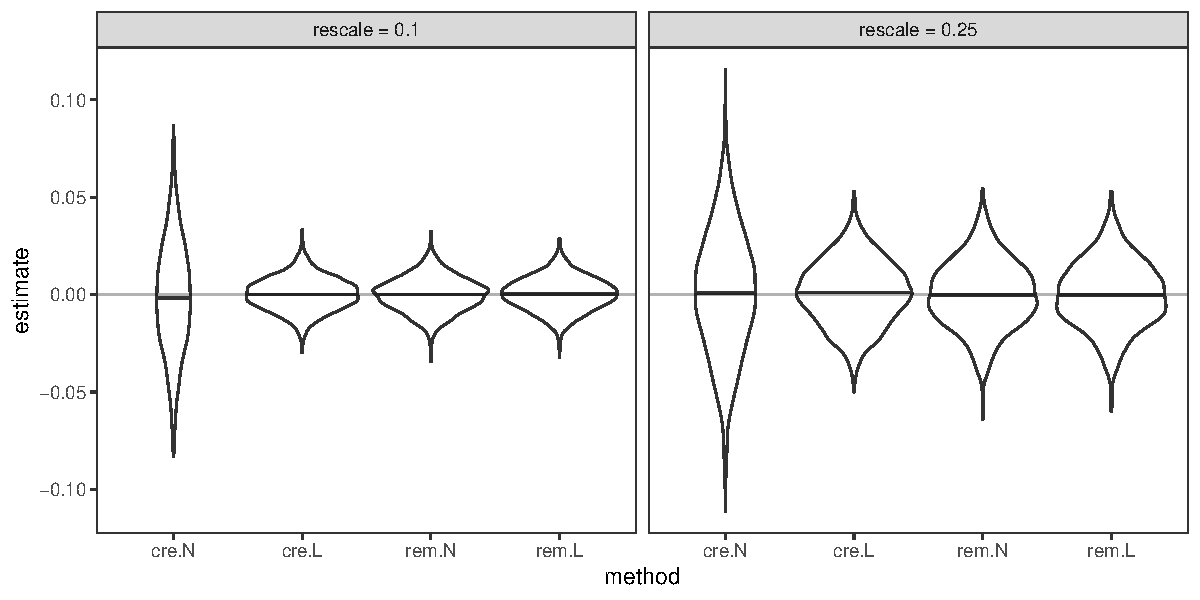
\includegraphics[width = \textwidth]{figures/RemReg_violin.pdf}
\caption{$2000$次蒙特卡洛重复、再随机化阈值$a=0.05$下的模拟} \label{fg::rerandomizationandancova}
\end{figure}


 


\section{结语}

再随机化以马氏距离作为平衡准则，也可将准则推广为$\bm{Z}$与$\bm{X}$的一般函数。例如，对$X_i = (x_{i1}, \ldots, x_{iK})\tran$的每个分量进行边际检验，只有在
\begin{equation}
\label{eq::marginal-testing-rerandomization}
\left | \frac{  \hat{\tau}_{xk} }{   \sqrt{  \frac{n}{n_1 n_0} S_{xk}^2       }  }   \right | \leq  a \quad ( k=1,\ldots, K )
\end{equation}
时才接受$\bm{Z}$，其中$a > 0$为预先指定的常数，$S_{xk}^2$是协变量$x_{ik}$的有限总体方差。例如，$a$可取标准正态分布的某个上分位点。基于准则\eqref{eq::marginal-testing-rerandomization}及其他准则的再随机化理论见\citet{zhao2021no}。 


对于连续结果，Fisher 的 ANCOVA 多年来一直是标准方法。即使线性模型误设，\citet{lin2013}的改进方法也有更好的理论性质。对于二元结果，常将观测结果对截距、处理指标和协变量作逻辑回归，用处理系数估计因果效应。但\citet{freedman2008randomization}表明，这种逻辑回归在潜在结果框架下的性质并不理想。即使模型正确，处理系数刻画的也是条件对数优势比（见第\ref{sec::logistic-regression}节），未必对应所关心的参数；模型错误时，更难解释。由前述讨论可知，若关注平均因果效应，仍可用\citet{lin2013}的估计量分析完全随机实验中的二元结果。\cite{guo2020generalized}推广了\citet{lin2013}的理论，允许在潜在结果框架下用广义线性模型构造平均因果效应估计量。  


\citet{lin2013}理论的其他推广涉及高维协变量。\citet{bloniarz2015lasso}考虑协变量数多于样本量的情形，建议将结果对截距、处理、协变量及交互项的 OLS 拟合，替换为最小绝对收缩与选择算子（LASSO）拟合\citep{tibshirani1996regression}。\citet{lei2018regression}考虑协变量数发散但不要求稀疏的情形，证明在一定正则条件下，\citet{lin2013}的估计量仍一致且渐近正态。\citet{wager2016high}提出用机器学习方法分析高维实验数据。 



\section{作业习题}

\paragraph{再随机化下的 Fisher 随机化检验}\label{hw::FRT-under-REM}

描述再随机化设计下的 Fisher 随机化检验方法。


\paragraph{马氏距离的不变性}\label{para::invariance-M}

证明引理\ref{lemma::invariance-mdistance}。 


\paragraph{再随机化下均值差的偏差性质}\label{hw::unbiasednessof-tauhat-rerandom}

假设从完全随机实验中抽取$\bm{Z} = (Z_1, \ldots, Z_n)$，仅当$\phi(\bm{Z}, \bm{X}) = 1$时接受该分配，其中$\phi$是预先指定的平衡准则。证明，若$n_1 = n_0$且
\begin{eqnarray}
\phi(\bm{Z}, \bm{X}) = \phi(\bm{1}_n-\bm{Z}, \bm{X}), \label{eq::symmetry}
\end{eqnarray}
则$\hat{\tau}$是$\tau$的无偏估计。验证：$n_1 = n_0$时，使用马氏距离的再随机化满足\eqref{eq::symmetry}。举出两个条件不成立时，$\hat{\tau}$对$\tau$有偏的反例。  


注：本题中的$\phi(\bm{Z}, \bm{X}) $可以是一般平衡准则。再随机化是$\phi(\bm{Z}, \bm{X})  =  I(M\leq a) $这一特例。


\paragraph{完全随机化下 $R^2$ 的等价表达}\label{para::r2-cre}

证明命题\ref{prop::rsquared-forms}。 



\paragraph{再随机化下线性调整估计量的方差分解}\label{hw::projection-po-onto-x}



证明
$$
S^2(1\mid X) = S_{Y(1)X} (S_X^2)^{-1} S_{XY(1)}
$$
其中$S_{XY(1)}$是$X_i$与$Y_i(1)$的有限总体协方差，$S_{Y(1)X} = S_{XY(1)}\tran$，$S_X^2$为$X_i$的有限总体协方差矩阵。写出$S^2(0\mid X) $和$S^2(\tau\mid X) .$的类似公式。



\paragraph{比较线性调整估计量族中的真实方差}\label{hw::compare-true-variance} 



证明$\hat{\tau}(\beta_1, \beta_0)$的方差可分解为
$$
\var\{ \hat{\tau}(\beta_1, \beta_0) \} 
=  
\var\{ \hat{\tau}( \tilde{\beta}_1, \tilde{\beta}_0) \}  
+
\var\{ \hat{\tau}(\beta_1, \beta_0) - \hat{\tau}(\tilde{\beta}_1, \tilde{\beta}_0) \}
$$
其中$\tilde{\beta}_1$和$\tilde{\beta}_0$分别是将$Y_i(1)$、$Y_i(0)$对$(1, X_i)$作 OLS 投影时，$X_i$的系数。 



注：\citet[][Example 9]{li2017general}推导了这一分解。由于$\var\{ \hat{\tau}(\beta_1, \beta_0) - \hat{\tau}(\tilde{\beta}_1, \tilde{\beta}_0) \}$始终非负，$\hat{\tau}( \tilde{\beta}_1, \tilde{\beta}_0)$在线性调整估计量族中按真实方差衡量是一个最优选择。   




\paragraph{Lin 回归调整估计量的等价表达}\label{para::lin-ols-covadj}

证明命题\ref{prop::lin-ols}。 

\paragraph{预测型与投影型估计量的等价性}\label{para::predictiveestimator}
证明 \eqref{eq::predictiveestimator} 和 \eqref{eq::projectiveestimator}。 
 
 
 \paragraph{线性调整估计量的代数表达}\label{para::reg-covariate-imbalance}

证明 \eqref{eq::linear-covariate-imbalance} 和 \eqref{eq::lin-covariate-imbalance}。 
 
 
 
\paragraph{ANCOVA 与协变量不平衡调整的关系}
\label{para::ancova-imbalance}

本题给出 ANCOVA 的一个结论，类似于\eqref{eq::lin-covariate-imbalance}。 

证明
$$
\hat{\tau}_\textsc{F} =\hat\tau  - \hat\gamma_\textsc{F}\tran \hat\tau_X,
$$
其中$ \hat\gamma_\textsc{F}$是将$Y_i$对$(1,Z_i, X_i)$作 OLS 回归时$X_i$的系数。 





 \paragraph{完全随机实验的回归调整与后分层}\label{para::lin=ps-discrete}
 
 证明命题\ref{prop::lin=ps-discrete}。 
 
 
注：有时$\hat{\tau}_{\textsc{ps}}$或$ \hat{\tau}_\textsc{L}$未必有良好定义。在这些情形下，把$\hat{\tau}_{\textsc{ps}}$与$ \hat{\tau}_\textsc{L}$视为相等。证明中可忽略这一复杂情况。 
 
%In a completely randomized experiment, we have a binary treatment indicator $Z$, an outcome $Y$, and a discrete covariate $X \in \{  1, \ldots, K \}$. We can use two methods to use covariates to improve estimation efficiency. 
%
%First, we can use the post-stratification estimator, pretending that the experiment is a stratified randomized experiment, conditional on $X$. This estimator is $\hat{\tau}_{\textsc{ps}}$. 
%
%Second, we can create $K-1$ dummy variables $\delta_{1i} = I(X_i=1), \ldots, \delta_{K-1,i} = I(X_i=K-1)$, and use Lin's estimator with covariates $\delta_1,\ldots, \delta_{K-1}$. This estimator is $\hat{\tau}_\textsc{L}$. 
%
%Show that $\hat{\tau}_{\textsc{ps}} = \hat{\tau}_\textsc{L}.$ Note that sometimes $\hat{\tau}_{\textsc{ps}}$ or $ \hat{\tau}_\textsc{L}$ may not be well-defined. In those cases, we treat $\hat{\tau}_{\textsc{ps}}$ and $ \hat{\tau}_\textsc{L}$ as equal. 


 
% \paragraph{Regression adjustment in the Fisher Randomization Test}
%This is a reanalysis of the LaLonde experimental data used in the lecture. In \texttt{FRTlalonde.R}, I conduct the Fisher randomization test using four test statistics. The Fisher randomization test can be more general with at least the following two additional strategies. Under the potential outcomes framework, {\it all potential outcomes and covariates are fixed numbers}. 
%
%
%First, we can use test statistics based on residuals from the linear regression. Run a linear regression of the outcomes on the covariates, and obtain the residuals (i.e., treat the residuals as the pseudo ``outcomes''). Then define the four test statistics based on the residuals. Conduct the Fisher randomization test using these four new test statistics. Report the corresponding $p$-values.
%
%
%Second, we can define the test statistic as the coefficient in the linear regression of the outcomes on the treatment and covariates. Conduct the Fisher randomization test using this test statistic. Report the corresponding $p$-value. 
%
%
%Why the five $p$-values from the above two strategies are exact $p$-values? Justify them. 


\paragraph{完全随机化下差异-差异估计量的性质}\label{hw::did-CRE}

本题补充第\ref{sec::difference-in-difference-CRE}节完全随机实验中双重差分估计量的细节。 

证明$\hat{\tau}(1,1) $是$\tau$的无偏估计，计算其方差，并证明$\hat{V}( 1,1 ) $是$\hat{\tau}(1,1) $真实方差的保守估计。什么情况下有$E\{\hat{V}( 1,1 ) \} = \var\{  \hat{\tau}(1,1)  \}$？



比较$\hat{\tau}(0,0) $与$\hat{\tau}(1,1) $的方差，证明
$$
\var\{ \hat{\tau}(0,0) \}  \geq \var\{  \hat{\tau}(1,1)  \}
$$
成立当且仅当
$$
2 \frac{n_0}{n} \beta_1 + 2\frac{n_1}{n} \beta_0 \geq 1,
$$
其中
$$
\beta_1 = \frac{\sum_{i=1}^n (X_i-\bar{X})\{  Y_i(1)-\bar{Y}(1) \}  }{  \sum_{i=1}^n (X_i-\bar{X})^2 },\quad
\beta_0 = \frac{\sum_{i=1}^n (X_i-\bar{X})\{  Y_i(0)-\bar{Y}(0) \}  }{  \sum_{i=1}^n (X_i-\bar{X})^2 }
$$
分别为将$Y_i(1)$和$Y_i(0)$对$(1,X_i)$作 OLS 回归时$X_i$的系数。 


注：\citet[][page 28]{gerber2012field}讨论了本题在$n_1=n_0.$时的特例。



\paragraph{Penn 奖学金实验的再分析}

 
重新分析宾州奖金实验数据。第\ref{chapter::stratification-poststratification}章的分析使用处理指标、结果和区组指标，现在需要使用其他所有协变量。 

在实验各层内进行回归调整，再合并调整后的估计量，估计平均因果效应。报告点估计、估计标准误和 95\% 基于实验数据，结合协变量进行回归调整并给出统计推断结果，与未调整结果进行比较分析。 
 

\paragraph{缺失结果下的统计推断}\label{hw::missing-y-experiments}

第\ref{sec::rem-reg-simulation}节的数据分析用简单填补法处理缺失结果，这具有一定任意性。 

分别用处理组和对照组的观测均值填补各组缺失结果，结论是否改变？

分别在处理组和对照组将观测结果对协变量作线性回归，用拟合值填补各组缺失结果，结论是否改变？ 

探讨不同缺失结果处理方法对统计推断的影响。 




\paragraph{推荐阅读}

本章标题与\citet{li2019rerandomization}相同，该文分别研究了再随机化和回归调整在随机实验设计与分析阶段中的作用。 


